% !TEX program = xelatex
\documentclass[twocolumn,superscriptaddress,english,showpacs,longbibliography]{revtex4-2}
\usepackage[colorlinks=true,urlcolor=blue,citecolor=blue,linkcolor=blue]{hyperref} 

\usepackage{svg}
\usepackage{amsmath}
\usepackage{graphicx}% Include figure files
\usepackage{textcomp}
\usepackage{bm}% bold math
\usepackage{color}
\usepackage{amssymb}
\usepackage{amsthm}
\usepackage{graphicx}
\usepackage{color}
\usepackage{mathrsfs}
\usepackage{float}
\usepackage{indentfirst}
\usepackage{txfonts}
\usepackage{algorithm}  
\usepackage{algpseudocode}  
\usepackage{balance}
\usepackage{flushend}
\usepackage{cleveref}
\usepackage{blkarray}
\usepackage{tikz}
\renewcommand{\algorithmicrequire}{\textbf{Input:}}  % Use Input in the format of Algorithm  
\renewcommand{\algorithmicensure}{\textbf{Output:}} % Use Output in the format of Algorithm  
\newtheorem{hyp}{Hypothesis}

\newcommand{\jinguo}[1]{[{\color{red}{JGL: #1}}]}
\newcommand{\ym}[1]{[{\color{blue}{YM: #1}}]}
\newcommand{\s}{\mathbf {s}}
\newcommand{\net}[1]{{\textsc{#1}}}
\newcommand{\vs}{{\mathbf{s}}}
\newcommand{\vn}{{\mathbf{n}}}
\newcommand{\argmin}{\mathop{\mathrm{argmin}}\limits}
\newcommand{\Eq}[1]{Eq.~(\ref{#1})}
\newcommand{\Fig}[1]{Fig.~\ref{#1}}

\begin{document}

\title{Crystal as a thermodynamic computer}

\author{Authors}
\email{xxx@xxx.com}
\affiliation{
    XXX
}

\begin{abstract}
\end{abstract}

\maketitle

\section{The implementation in Rydberg atoms array}\label{physical-model-rydberg-atoms-array}
Let us consider a Rydberg atoms array with a two dimensional embedding. The coordinate of the atom $v$ is denoted as $\mathbf{r}_v$.
The Rydberg Hamiltonian~\cite{Nguyen2023} is defined as
\begin{equation}
    H_{\text{Ryd}} = \sum_v \dfrac{\Omega_v}{2} \sigma^x_v -\sum_v \Delta_v n_v + \sum_{v < w}  V_{\text{Ryd}}(|\overrightarrow{\mathbf{r}_v} -\overrightarrow{\mathbf{r}_w}|)n_v n_w,
\end{equation}
where $\Omega_v$ is the Rabi frequency, $\Delta_v$ is the detuning,
$n_v = \dfrac{1}{2}(1 - \sigma^z_v)$ is the number operator, and
$V_{\text{Ryd}}(|\overrightarrow{\mathbf{r}_v} - \overrightarrow{\mathbf{r}_w}|) = C_6/|\overrightarrow{\mathbf{r}_v} - \overrightarrow{\mathbf{r}_w}|^6$
is the Rydberg interaction potential.

In the following, we will show the classical part of the Rydberg Hamiltonian encodes an independent set problem~\cite{Moore2011} on a unit disk graph.
In graph theory, an independent set is a set of vertices in a graph, no two of which are adjacent.
Here, we restrict the graph to be a two dimensional unit disk graph $G=(V, E)$, a geometric graph with two dimensional embedding, such that two vertices $u, v \in V$ are connected if and only if they are within the unit radius, i.e. $|\mathbf r_u - \mathbf r_v| < r_B$. This reflects the blockade phenomenon in Rydberg atoms arrays, where two atoms within blockade radius $r_B$ can not excite to the Rydberg state simultaneously due to the strong Rydberg interaction potential. Let us idealize the energy model by treating the blockade interaction between two atoms as infinity if two atoms are within blockade radius, zero otherwise. Then the energy model becomes
\begin{equation}
H_{\text{MWIS}} = -\sum_{v \in V}\Delta_v n_v + \sum_{(u, v) \in E} \infty n_u n_v.
\end{equation}
The ground state of which encodes the maximum weight independent set (MWIS) problem, and $\Delta_v$ is the weight associated with vertex $v \in V$. Whenever we have a atom in the Rydberg state in the ground state of $H_{\text{WMIS}}$, we add the vertex associated with that atom to the maximum independent set.

\section{Gadget finding}
Given a target logic gate, the goal is to find a graph $G = (V, E)$ and weights associated with vertices $\{\Delta_v \mid v\in V\}$ such that the WMIS problem of this graph encodes this gate.

Let $\mathcal{M}$ be the set of all maximal independent sets of $G$, where a maximal independent set is an independent set that is not a subset of any other independent set.
Each $\mathbf n \in \mathcal{M}$ is associated with an energy $H_{\text{WMIS}}(\mathbf n) = -\sum_v \Delta_v n_v$. We denote the target states with minimum energy as $\mathcal{M}_{\text{min}} \subseteq \mathcal{M}$. We can express the linear programming problem as
\begin{equation}\label{eq:lp}
    \begin{split}
        &\min_{\boldsymbol{\Delta} \in \mathbb{R}^{|V|}} 0\\
        &\sum_i n_i' \Delta_i < \sum_i n_i \Delta_i, \forall \mathbf n \in \mathcal{M}_{\text{min}}, \mathbf n' \in \mathcal{M} \setminus \mathcal{M}_{\text{min}}\\
        &\sum_i n_i \Delta_i = \sum_i n_i' \Delta_i, \forall \mathbf n, \mathbf n' \in \mathcal{M}_{\text{min}}
    \end{split}
\end{equation}
Note that the constraints are all linear. The less constraints and equality constraints can be easily transformed into inequality constraints by adding ancilla variables.
The possible choice of $S_{\text{min}}$ grows exponentially as the number of ancilla vertices increases, which limits the capability of this method.
\jinguo{We focus on the general graphs first.}

In the following, we restrict the graph to be two dimensional grid graphs, the unit distance can be arbitrary. A graph configuration can be denoted as a boolean mask $M\in \{0, 1\}^{m\times n}$.
\jinguo{Then the unit disk graphs.}

\subsection{Energy based universal computation with Rydberg atoms
array}\label{energy-based-universal-computation-with-rydberg-atoms-array}

The classical Rydberg Hamiltonian is universal for classical computation, since the NOR gate can be implemented using the Rydberg Hamiltonian (subfigure
c below). The NOR gate is a universal gate for classical computation.
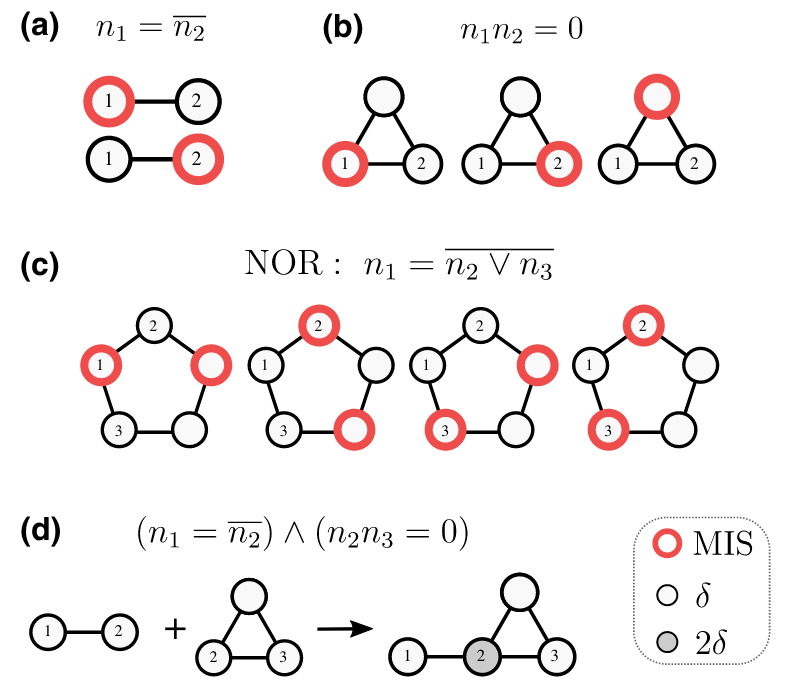
\includegraphics[width=\columnwidth]{../notes/images/gadgets.png}

The conjunction of gates can be implemented by ``gluing'' the Rydberg
atoms together (subfigure d below). The weights are added together.

For more logic gates, please check the GitHub repository
\href{https://github.com/QuEraComputing/UnitDiskMapping.jl/blob/main/test/logicgates.jl}{UnitDiskMapping.jl}.

\subsection{The Rule 110 Gadget}\label{the-rule-110-gadget}

We can encode the Rule 110 CA into a Weighted Maximum
Independent Set Problem, with blue vertices assigned a weight of 1 and
red vertices assigned a weight of 2, as follows.

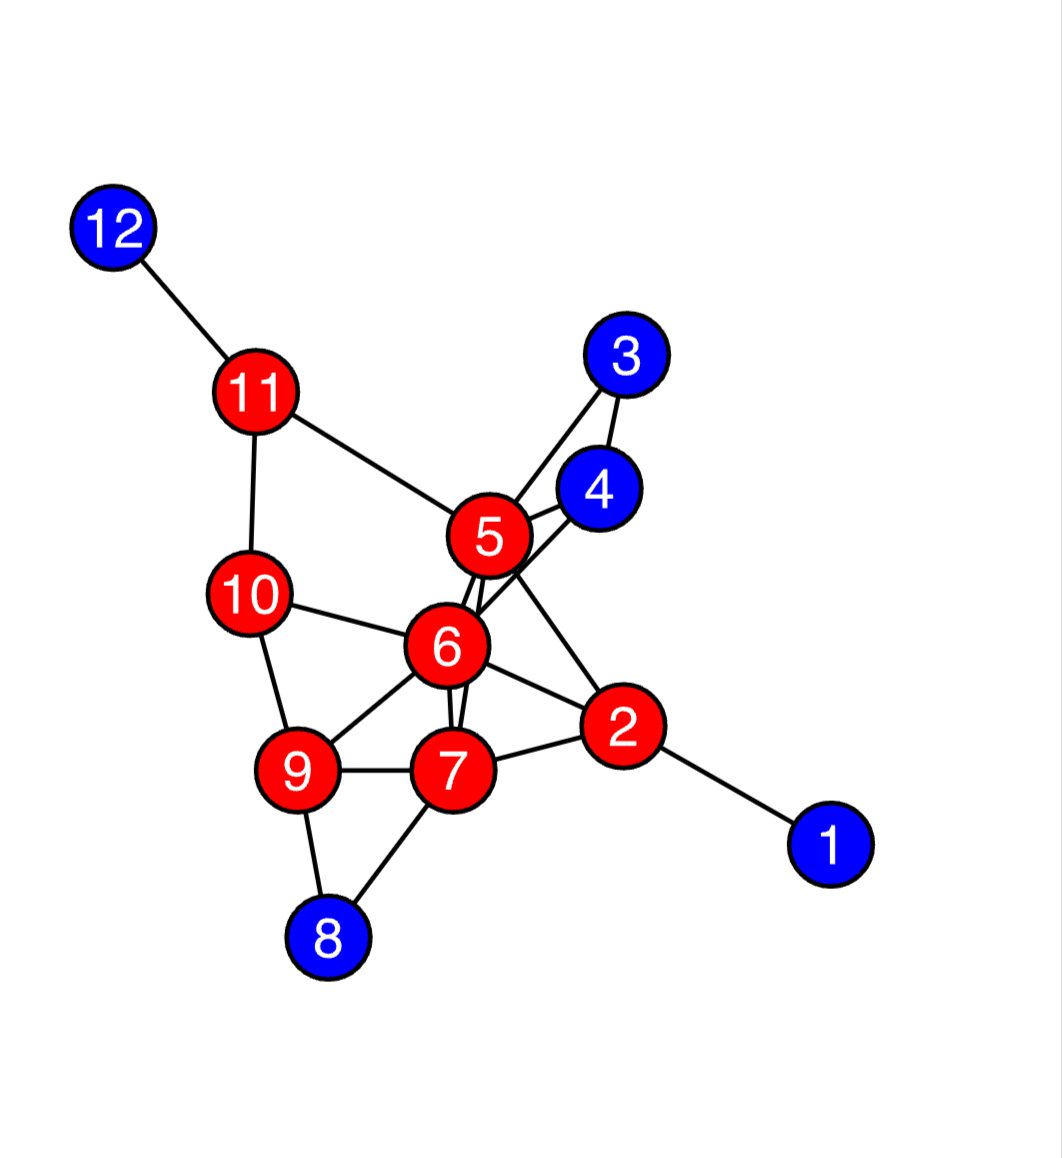
\includegraphics[width=0.6\columnwidth]{../notes/images/image.png}

This graph can be embedded into a grid graph, where two vertices are
connected if and only if their Euclidean distance is no more than $2$.

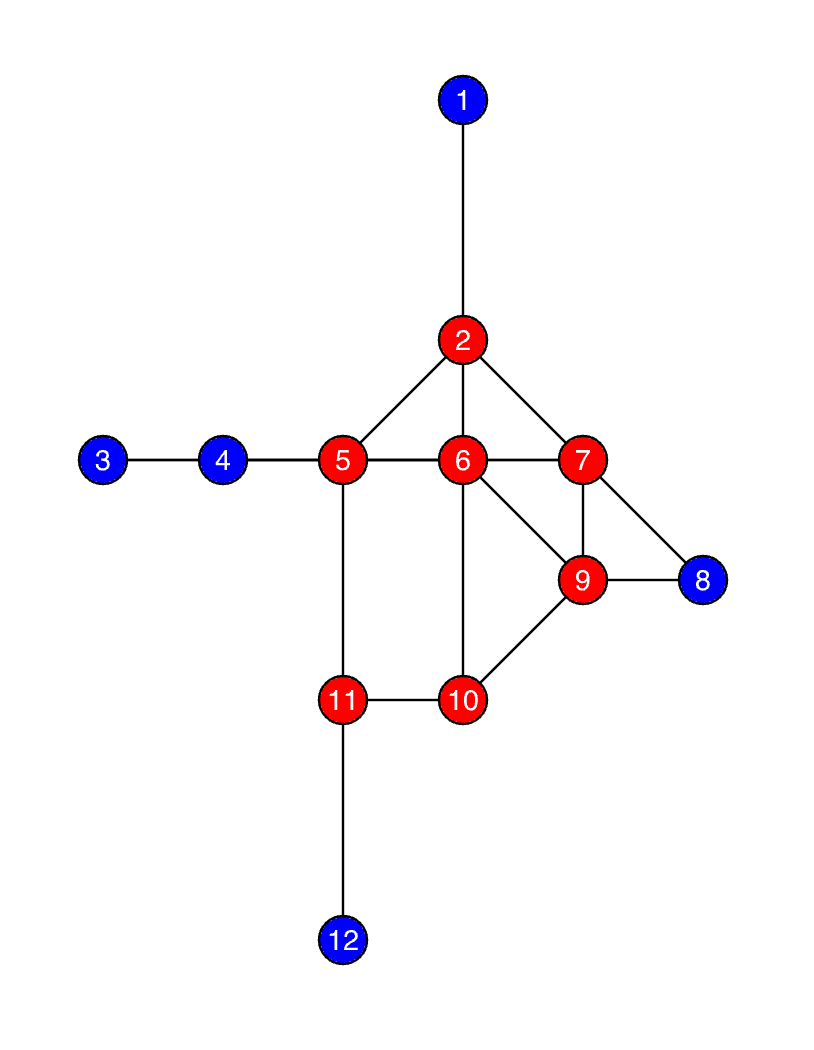
\includegraphics[width=0.7\columnwidth]{../notes/images/image-1.png}

The correspondence between the Maximum Weighted Independent Set (MWIS)
Solution and Rule 110 is as follows:

The states of vertex \textbf{1}, vertex \textbf{3}, and vertex
\textbf{8} represent the states of the \textbf{middle}, \textbf{left},
and \textbf{right} cells of the automata's \textbf{input},
respectively. If the input value of a cell is 1, then the corresponding
vertex must be in the MWIS solution; otherwise, it is not. Vertex
\textbf{12} corresponds to the automata's \textbf{output}. If the
automata output is 1, then vertex 12 is in the MWIS solution;
otherwise, it is not.

In the automata diagram, the above gadget is equivalent to:
There are exactly \textbf{8} different MWIS solutions in this graph (the
weighted size of each MWIS solution is 7), each corresponding to one of
the \textbf{8} possible outputs of the automata. We list them as
follows.
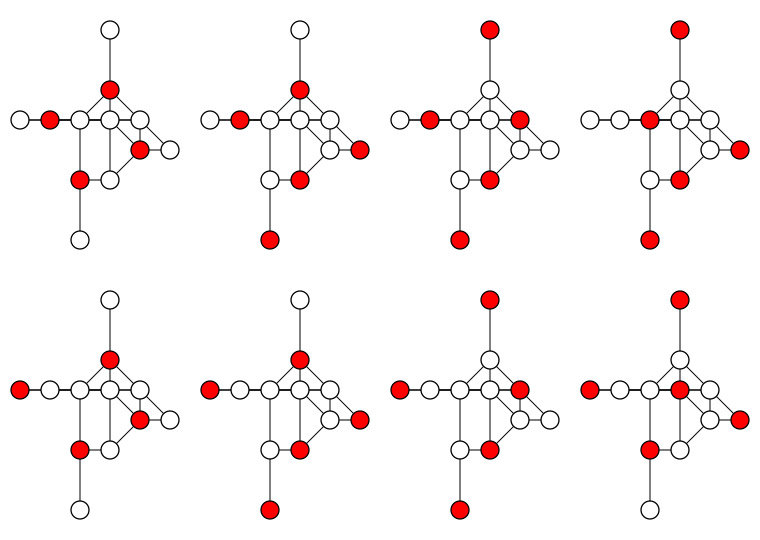
\includegraphics[width=\columnwidth]{../notes/images/gadget110.png}

Utilizing copy gadget and cross gadget~\cite{Nguyen2023}, we construct a \textbf{Surface Programmable Material} with open boundary conditions as follows.

\begin{figure}
\centering
\includesvg[width=\columnwidth]{../notes/images/rule110transvarient.svg}
\caption{Alt text}
\end{figure}

The above gadget depicts a two-layer CA. The vertices in
blue, red, green and black have weights of 1, 2, 3 and 4, respectively.
In the automata diagram, the above gadget is equivalent to:

\jinguo{Tasks:
\begin{enumerate}
    \item Implement the gadget design algorithm in \Cref{eq:lp}.
    \item Use the algorithm to search for all two-bit logic gates and CA rules.
    \item Generate all unit disk graphs with size < 15 (please check \href{https://github.com/GiggleLiu/SmallGraphs}{small graph zoo}).
    \item Use the algorithm to search for MWIS gadgets on unit disk graphs.
\end{enumerate}
}

\begin{acknowledgments}
    %We thank Lei Wang, Madelyn Cain and XXX for helpful discussions on the simulation methods.
\end{acknowledgments}

%\bibliographystyle{apsrev4-1}
\bibliography{refs.bib}

\appendix

\end{document}
